
\section{Making Modeling Choices}
\label{sec:modeling-choices}

\subsection{Computational box} \label{subsect:coords}
\optsection{Computational box}
\optseealso{Grid}

PISM does all simulations in a computational box\index{PISM!computational box} which is rectangular in the PISM coordinates.

The coordinate system has horizontal coordinates $x,y$ and a vertical coordinate $z$.  The $z$ coordinate is measured positive upward from the base of the ice and it is exactly opposite to the vector of gravity.  The surface $z=0$ is the base of the ice, however, and thus is usually not horizontal in the sense of being parallel to the geoid.   The surface $z=0$ is the base of the ice both when the ice is grounded and when the ice is floating.

Bed topography is, of course, allowed.  In fact, when the ice is grounded, the true physical vertical coordinate $z'$, namely the coordinate measure relative to a reference geoid, is given by $z'=z+b(x,y)$ where $b(x,y)$ is the bed topography.  The surface $z'=h(x,y)$ is the surface of the ice.

In the grounded case the equation $h(x,y)=H(x,y)+b(x,y)$ always applies if $H(x,y)$ is the thickness of the ice.  In the floating case, the physical vertical coordinate is $z'=z-(\rho_i/\rho_s) H(x,y)$ where $\rho_i$ is the density of ice and $\rho_s$ the density of sea water.  Again $z=0$ is the base of the ice, which is the surface $z' = -(\rho_i/\rho_s) H(x,y)$.  The surface of the ice is $h(x,y) = (1-\rho_i/\rho_s) H(x,y)$.  All we know about the bed elevations is that they are below the base of the ice when the ice is floating.  That is, the \emph{flotation criterion} $-(\rho_i/\rho_s) H(x,y) > b(x,y)$ applies.

The computational box can extend downward into the bedrock.  As $z=0$ is the base of the ice, the bedrock corresponds to negative $z$ values regardless of the sign of its true (i.e.~$z'$) elevation.

The extent of the computational box, along with its bedrock extension downward, is determined by four numbers \t{Lx}, \t{Ly}, \t{Lz}, and \t{Lbz} (see Figure \ref{fig:rectilinearbox}.).  The first two of these are half-widths and have units of kilometers when set by options or displayed.  The extent of the computational box for the ice and bedrock is directly controlled by the following options. 

\begin{center}
  \begin{tabular}{llp{0.7\linewidth}}
    \\\toprule
    \textbf{Option} & \textbf{Meaning}
    \\\midrule
    \txtopt{Lx}{(km)} & Half-width of the computational domain (in the $x$-direction) \\
    \txtopt{Ly}{(km)} & Half-width of the computational domain (in the $y$-direction) \\
    \txtopt{Lz}{(meters)} & Height of the computational domain in the ice \\
    \txtopt{Lbz}{(meters)} & Depth of the computational domain in the bedrock thermal layer
    \\\bottomrule
  \end{tabular}
\end{center}

\begin{figure}[ht]
\centering
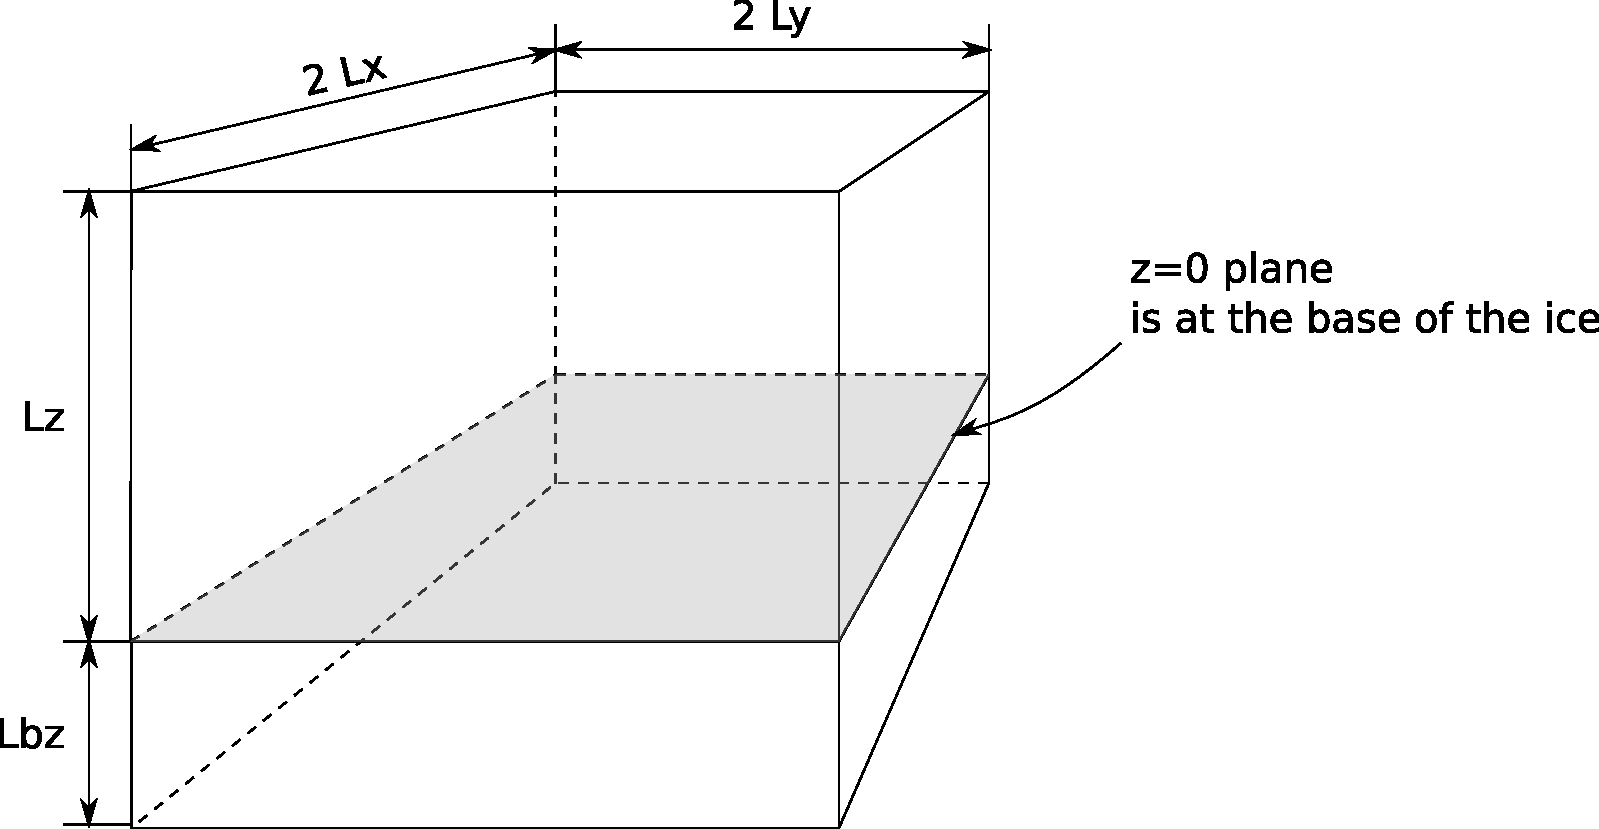
\includegraphics[width=4.0in,keepaspectratio=true]{rectilinearbox}
\caption{PISM's computational box.}
\label{fig:rectilinearbox}
\end{figure}


\subsection{Spatial grid}
\label{subsect:grid}
\optsection{Grid!space}

The PISM grid\index{PISM!grid} covering the computational box is equally spaced in horizontal ($x$ and $y$) directions.  Vertical spacing is quadratic by default (see below) but optionally a different spacing scheme can be chosen.  (Choose with options \txtopt{z_spacing}{[quadratic, equal]} and \txtopt{zb_spacing}{[quadratic, equal]}.)

The grid is described by four numbers, namely the number of grid points \texttt{Mx} in the $x$ direction, the number \texttt{My} in the $y$ direction, the number \texttt{Mz} in the $z$ direction within the ice, and the number \texttt{Mbz} in the $z$ direction within the bedrock thermal layer.  These are specified by options \intextoption{Mx}, \intextoption{My}, \intextoption{Mz}, and \intextoption{Mbz}, respectively. The defaults are 61, 61, 31, and 1, respectively.

Note that \texttt{Mx}, \texttt{My}, \texttt{Mz}, and \texttt{Mbz} all indicate the number of grid \emph{points}.  The number of grid \emph{spaces} are one less, thus 60, 60, 30, and 0 in the default case.  The lowest grid point in a column of ice, at $z=0$, coincides with the highest grid point in the bedrock, so \texttt{Mbz} must always be at least one and \texttt{Mbz}$>1$ is required to use the bedrock thermal model.  Note that this option is unrelated to the bed deformation model (glacial isostasy model); see option \texttt{-bed_def} for that.

In the quadratic case, the spacing near the ice/bedrock interface is about four times finer than it would be with equal spacing for the same value of \texttt{Mz} (or \texttt{Mbz}), while the spacing near the top (or bottom) is correspondingly coarser. For a detailed description of the spacing of the grid, see the documentation on \texttt{IceGrid::compute_vertical_levels()} in the PISM class browser.

When a thermal bedrock layer is used, the distance \texttt{Lbz} is controlled by the \texttt{-Lbz} option.

If one initializes PISM from a saved model state using \t{i} then the input model state controls the parameters \t{Mx}, \t{My}, \t{Mz}, and \t{Mbz}.  For instance, the command

\begin{verbatim}
$  pismr -i foo.nc -y 100
\end{verbatim}

\noindent should work fine if \texttt{foo.nc} was a valid PISM model file.  The command

\begin{verbatim}
$  pismr -i foo.nc -Mz 201 -y 100
\end{verbatim}

\noindent will give a warning that ``\texttt{PISM WARNING: ignoring command-line option '-Mz'}'' because \texttt{-i} input files take precedence.

Otherwise, one is allowed to specify the grid when PISM is started.  In particular, the user should specify the grid when using \texttt{-boot_from} or when initializing a simplified-geometry experiment or a verification test, though defaults are generally present in the latter cases.  See sections \ref{sect:start} and \ref{sect:boot} for examples and explanation.

\subsection{Model time}
\label{sec:time}
\optsection{Grid!time}

The following command-line options control PISM time.

\begin{tabular}{lp{0.8\linewidth}}\\
\toprule
\textbf{Option} & \textbf{Meaning}\\
\midrule
\txtopt{y}{(years)} & Number of model years to run.\\
\txtopt{ys}{(years)} & Model year at which to start the run.  Also resets the model time, ignoring any time in the input file.\\
\txtopt{ye}{(years)} & Model year at which to end the run.\\
\bottomrule
\end{tabular}

The default value for the end year is the start year (\texttt{-ys} or initialized model time from file) plus the default or given (\texttt{-y}) run length.  If both \texttt{-ys} and \texttt{-ye} are used then the run length is set to the difference.  Using all three of \texttt{-ys}, \texttt{-y} and \texttt{-ys} is not allowed.


\subsection{Diagnostic computations}  As a diagnostic example, consider the second of these two runs:

\begin{verbatim}
pisms -y 200e3 -o eisIIA200k.nc
pismr -i eisIIA200k.nc -y 0 -o eisIIA200k_diag.nc -o_size big
\end{verbatim}

\noindent The result of this zero-length, ``\texttt{-y 0}'', run is a NetCDF file \texttt{eisIIA200k_diag.nc} which contains the full three-dimensional velocity field in the scalar NetCDF variables \texttt{uvel}, \texttt{vvel}, and \texttt{wvel}, as well as many other variables.

This diagnostic mode is most frequently associated to the modeling of ice shelves and ice streams.  Subsection \ref{sect:ross} describes using \texttt{pross} to model the Ross ice shelf \cite{MacAyealetal}.  Verification tests I and J, section \ref{sect:verif}, are diagnostic calculations using the SSA.

Note that the NetCDF model state saved by PISM at the end of an \emph{evolution} run does not, by default, contain the three-dimensional velocity field.  Instead, it contains just the variables which are needed to restart the run, especially the ice geometry and temperature field.  One can also force PISM to save all the supported diagnostic quantities at the end of a time-stepping run using the option \texttt{-o_size big}.


\subsection{Computing ice age} \label{subsect:age}
\optsection{Computing ice age}

By default, PISM does not compute the age of the ice\index{PISM!modeling the age of the ice} because it does not directly impact ice flow using the default flow laws.   It is very easy to turn on.  Just set \intextoption{age}.

\subsection{Setting up PISM boundary (atmosphere, surface and ocean) models}
\label{sec:boundary-models}

Setting up PISM's boundary models requires selecting one model of each kind and zero or more ``model modifiers''; selected models and modifiers are chained as in Figure~\ref{fig:climate-input-data-flow}. Command-line options \texttt{-atmosphere}, \texttt{-surface} and \texttt{-ocean} take a comma-separated list of keywords as an argument; the first keyword \emph{has} to correspond to a model, the rest can be modifiers. Any of these options can be omitted to use the default atmosphere, surface or ocean model, although using a modifier requires specifying a model.

For example,
\begin{verbatim}
$ pismr -i foo.nc -atmosphere searise_greenland,forcing \
        -dTforcing delta_T.nc -surface pdd
\end{verbatim}%$
chooses a combination of SeaRISE-Greenland atmosphere model (see below),  ice-core derived temperature forcing, a PDD local surface mass balance model, and a default (constant) ocean model.

Each of PISM boundary model types currently has one ``modifier'' available; the corresponding keyword is \texttt{forcing}. Please see below for details.

\begin{enumerate}
\optsection{Climate (boundary) models!\texttt{-atmosphere} [searise_greenland, constant, temp_lapse_rate, forcing]}
\item \textbf{PISM atmosphere models.}
\begin{itemize}
  \item \emph{SeaRISE-Greenland} (\texttt{searise_greenland}, the default)

    This atmosphere model implements a longitude, latitude and elevation dependent near-surface air temperature parameterization and a cosine yearly cycle described in \cite{Faustoetal2009} and uses a constant in time ice-equivalent snow precipitation field (in units of thickness per time, variable \texttt{snowprecip}) that is read from an input file.

    The parameterization is controlled by configuration parameters with the \texttt{snow_temp} prefix.

    In addition to the temperature parameterization it implements the SeaRISE-Greenland formula for paleo-precipitation from present; a 7.3\% change of precipitation rate for every one degree Celsius of temperature change \cite{Huybrechts02} (turn on using the \intextoption{paleo_precip} option).

    Please see \url{http://websrv.cs.umt.edu/isis/index.php/Model_Initialization#Greenland} for details.

    It expects variables \texttt{snowprecip}, latitude and longitude to be present in an input file.

 \item \emph{Constant in time} (\texttt{constant})

    This atmosphere model reads the snow precipitation (variable \texttt{snowprecip}) and the mean annual near-surface air temperature (variable \texttt{temp_ma}) and provides them to a surface model.
  \item \emph{Constant precipitation using a temperature lapse rate} (\texttt{temp_lapse_rate})
    
    This atmosphere model also uses a constant snow precipitation field (\texttt{snowprecip}) and requires the mean annual near-surface air temperature (\texttt{temp_ma}) to be present in an input file. In addition to this, it dynamically corrects air temperature using a location-independent elevation lapse rate specified using the \intextoption{lapse_rate} command-line option (in units of degrees Celsius per meter).
 \end{itemize}

  The atmosphere \texttt{forcing} modifier implements temperature forcing using scalar offsets and also a mechanism applying precipitation and mean annual temperature anomalies.
  \begin{itemize}
  \item \fileopt{dTforcing} specifies a file containing scalar temperature offsets (variable \texttt{delta_T}), 
  \item \fileopt{anomaly_temp_ma} specifies a file containing spatially-variable mean annual near-surface air temperature anomalies (variable \texttt{temp_ma_anomaly}), and
  \item \fileopt{anomaly_precip} specifies a file containing spatially-variable ice-equivalent precipitation anomalies (in units of thickness per time, variable \texttt{snowprecip_anomaly}).
  \end{itemize}

  Options \texttt{-anomaly_temp_ma} and \texttt{-anomaly_precip} can be used to set up a PISM run using a GCM output, essentially achieving one-way coupling.

  Note that only one air temperature forcing mechanism can be used at any time.

\optsection{Climate (boundary) models!\texttt{-surface} [simple, constant, pdd, forcing]}
\item \textbf{PISM surface (snow) process models}

\begin{itemize}
  \item \emph{The ``invisible'' model} (\texttt{simple}, the default)

    This is the simplest ``surface model'' available in PISM. Its job is to re-interpret  precipitation as mass flux into the ice and mean annual near-surface air temperature as the temperature of the ice at the ice surface (below firn) (see \cite{Hock05}, for example). This implies that there is no melt as long as the precipitation field  is non-negative.

    However primitive it may be, this model can be useful; modeling Antarctica is one example.
  \item \emph{Constant in time} (\texttt{constant})

    This surface model reads constant in time top surface boundary conditions and provides them to the ice dynamics model (see table \ref{tab:ice-dynamics-bc}). When PISM is used with this model, variables \texttt{artm} (ice temperature at the ice surface but below firn) and \texttt{acab} (top surface mass flux into the ice) are expected to be present in an input file.

    Note: this surface model \emph{ignores}  the atmosphere model selection made using the \texttt{-atmosphere} option.

  \item \emph{Local mass balance (PDD)} (\texttt{pdd}) \index{positive degree day model} \index{PDD (positive degree day model)} \index{PISM!default positive degree day model} 

   The default PDD used by PISM, turned on by option \texttt{-surface pdd}, is based on \cite{CalovGreve05} and EISMINT-Greenland intercomparison (section \ref{sec:eismint-greenland} and \cite{RitzEISMINT}). It also implements latitude- and mean July temperature dependent ice and snow factors using formulas in \cite{Faustoetal2009}.

   Our PDD implementation is meant to be used with an atmosphere model implementing a cosine yearly cycle such as \texttt{searise_greenland}, but is not restricted to parameterizations like this one. A PDD generally adds ``white noise'' to the seasonal cycle to simulate additional daily variability associated to the vagaries of weather.  This additional random variation is quite significant, as the seasonal cycle may never reach the melting point but that point may be reached with some probability, in the presence of the daily variability, and thus melt may occur.  Concretely, a normally-distributed, mean zero random temperature increment is added to the seasonal cycle.  The standard deviation of the daily variability is controlled by the \intextoption{pdd_std_dev} option (and the corresponding config. parameter), and defaults to 2.53 degrees \cite{Faustoetal2009}. There is no assumed spatial correlation of daily variability.

The number of positive degree days is computed as the magnitude of the temperature excursion above $0\!\phantom{|}^\circ \text{C}$ multiplied by the duration (in days) when it is above zero.  In PISM there are actually two methods for computing the number of positive degree days.  The first computes only the expected value, by the method described in \cite{CalovGreve05}.  This is the default when a PDD is chosen (i.e.~option \texttt{-surface pdd}).  The second is a monte carlo simulation of the white noise itself, chosen by adding the option \intextoption{pdd_rand}.  This monte carlo simulation adds the same daily variation at every point, though the seasonal cycle is (generally) location dependent.  If repeatable randomness is desired use \intextoption{pdd_rand_repeatable} instead of \texttt{-pdd_rand}.

The number of positive degree days is multiplied by a coefficient (config parameter \texttt{pdd_factor_snow}) to compute the amount of snow melted.  Of the melted snow, a fraction (\texttt{pdd_refreeze}) is kept as ice.  This ice, plus all unmelted snow (already measured as ice-equivalent) is added to the mass balance, unless the number of positive degree days exceeds that required to melt all of the snow.  In this latter case, in which there are excess positive degree days available for melting, the excess is multiplied by a coefficient (\texttt{pdd_factor_ice}) to compute how much ice is melted.  In this case actual ablation occurs at that location.

In addition to this, one can use latitude- and July-air-temperature-dependent Greenland PDD model parameters $\beta_{\mathrm{ice}}$ and $\beta_{\mathrm{snow}}$ (formulas (6) and (7) in \cite{Faustoetal2009}) by adding the \intextoption{pdd_fausto}  option. See also configuration parameters with the \texttt{pdd_fausto} prefix..
\end{itemize}

The \texttt{forcing} modifier implements a surface mass balance adjustment mechanism forcing ice thickness to a target distribution at the end of the run; option \fileopt{force_to_thk} selects a file containing the target ice thickness field. Option \intextoption{force_to_thk_alpha} sets the $\alpha$ parameter. See the documentation  of \texttt{PSForceThickness::ice_surface_mass_flux()} for details.

\optsection{Climate (boundary) models!\texttt{-ocean} [constant, forcing]}
\item \textbf{PISM ocean models}
PISM includes one simple ocean model: \texttt{constant}, providing constant (both in time and space) mass flux into the ocean and sea level elevation to PISM's ice flow core. The mass flux is controlled by the\\ \texttt{ocean_sub_shelf_heat_flux_into_ice} configuration parameter and the assumption that the mass flux is proportional to heat flux into ice.

  The ocean \texttt{forcing} modifier implements sea level forcing. The command-line option \fileopt{dSLforcing} is used to specify the file containing sea level offsets:
\begin{verbatim}
$ pismr -i in.nc -ocean constant,forcing -dSLforcing delta_SL.nc
\end{verbatim}%$
uses \texttt{delta_SL.nc}
\end{enumerate}
  
\subsection{Flotation criterion and mask} \label{subsect:floatmask}  The most basic decision about ice dynamics made internally by PISM is whether to apply the ``flotation criterion'' to determine whether the ice is floating on the ocean or not.  In an evolution run this decision is made at each time step and the result is stored in the \t{mask}.

The possible values of the \t{mask}\index{mask} are given in Table \ref{tab:maskvals}.  The mask does not by itself determine ice dynamics.  For instance, when ice is floating (either value \texttt{MASK_FLOATING} or \texttt{MASK_FLOATING_AT_TIME_0}) the usual choice for ice dynamics is SSA, but the user can choose not to apply that model by not using either option \texttt{-ssa_floating_only} or \texttt{-ssa_sliding}.

\begin{table}[ht]
\centering
\caption{The PISM mask\index{mask}, in combination with user options, determines the dynamical model.}\label{tab:maskvals} 
\small
\begin{tabular}{p{0.25\linewidth}p{0.65\linewidth}}
\\\toprule
\textbf{Mask value} & \textbf{Meaning}\\\midrule
1=\texttt{MASK_SHEET} & ice is grounded (and only the SIA is always applied) \\
2=\texttt{MASK_DRAGGING_SHEET} & ice is grounded (and the SSA is applied if option \texttt{-ssa} is given) \\
3=\texttt{MASK_FLOATING} & ice is floating (and the SSA is applied if option \texttt{-ssa} is given) \\
7=\texttt{MASK_FLOATING_AT_TIME_0} & same as \texttt{MASK_FLOATING}, but the grid point was ice free ocean at initialization of the model by \texttt{-boot_from}; ice with this value will calve off if option \texttt{-ocean_kill} is given.
\\\bottomrule
\end{tabular}
\normalsize
\end{table}

Assuming the geometry of the ice evolves (which can be turned off by option \texttt{-no_mass}), and assuming an ocean exists (which can be turned off by option \texttt{-dry}), then at each time step the mask can change.  Ice which becomes floating is marked as \texttt{MASK_FLOATING} while ice which becomes grounded is either marked as \texttt{MASK_SHEET} or \texttt{MASK_DRAGGING}.  The latter case occurs if the option \texttt{-ssa_sliding} is used, while otherwise all points are marked \texttt{MASK_SHEET}.

\subsection{Calving}
\label{sec:calving}
\optsection{Calving}

PISM includes two very basic calving mechanisms activated using options in Table \ref{tab:calving}.  Other more physically-motivated calving laws (e.g.~\cite{Levermannetalsubmitted}) is planned for future versions of PISM.
\begin{table}
  \centering
  \begin{tabular}{lp{0.7\linewidth}}
    \\\toprule
    \textbf{Option} & \textbf{Description}
    \\\midrule
    \intextoption{float_kill} & All floating ice is calved off immediately.\\
    \intextoption{ocean_kill} & All ice flowing into grid cells marked as \texttt{MASK_FLOATING_AT_TIME_0} is calved off.
    \\\bottomrule
 \end{tabular}
  \caption{Calving options}
  \label{tab:calving}
\end{table}

\subsection{Rheology}
\label{sec:rheology}
\optsection{Rheology}

In the polythermal (default) mode of PISM there is only one choice of the flow law: the Glen-Paterson-Budd-Lliboutry-Duval \cite{AschwandenBlatter,LliboutryDuval1985,PatersonBudd}. 

Note that a ``flow law'' here means the function $F(\sigma,T,P,d)$ in the relation
	$$\dot \eps_{ij} = F(\sigma,T,P,d)\, \sigma_{ij}'$$
where $\dot \eps_{ij}$ is the strain rate tensor, $\sigma_{ij}'$ is the stress deviator tensor, $T$ is the ice temperature, $\sigma^2 = \frac{1}{2} \|\sigma_{ij}'\|_F$ so $\sigma$ is the second invariant of the stress deviator tensor, $P$ is the pressure, and $d$ is the grain size.  That is, we are addressing isotropic flow laws only, and one can choose the scalar function.  Note that the inverse form of such a flow law in needed for ice shelves and ice streams:
	$$\sigma_{ij}' = 2 \nu(\dot\eps,T,P,d)\,\dot \eps_{ij} $$
Here $\nu(\dot \eps,T,P,d)$ is the effective viscosity.  The need for this inverse form of the flow law explains the ``hybrid'' law \texttt{-ice_type hybrid}, because the inverse form of the Goldsby-Kohlstedt law is unknown.

The command-line option \intextoption{e} sets the flow enhancement factor and can be used with any flow law.  It alters the SIA flow law to be
	$$\dot \eps_{ij} = e\, F(\sigma,T,P,d)\, \sigma_{ij}'.$$

Command-line option \intextoption{ice_type} control the flow law in the \texttt{-cold} mode.  Arguments to \texttt{-ice_type} are in table \ref{tab:flowlaw} below.

Some ice types are customizable, run with \texttt{-help} to see all the customizable options for your chosen ice type (since \texttt{-help} displays many options, it is often useful to grep the output, as in \texttt{pisms -ice_type custom -help | grep ice_}).

A common use of the \texttt{custom} ice type is to directly specify the hardness parameter in an ice shelf study.  The viscous stress term in the $x$-component (for example) of the SSA equations for ice shelves and ice streams is
	$$\ddx{}\left(2\nu H\left(2\ddx{u} + \ddy{v}\right)\right)$$
where 
	$$\nu = \frac{\bar B}{2} \left[\left(\ddx{u}\right)^2 + \left(\ddy{v}\right)^2 +
  \frac{1}{4} \left(\ddy{u} + \ddx{v}\right)^2 + \ddx{u}\ddy{v}\right]^{(1-n)/(2n)}.$$
Generally $\bar B$ is computed by a vertical-integral of a function of the temperature field, but it is constant for isothermal ice.  If \intextoption{ice_custom_hardness} is used then $\bar B$ is set to the given value.  The value should have units of Pa $\text{s}^{1/n}$ where $n$ is the Glen exponent (see \texttt{-ice_type}).  Note that the cold-mode ice type (\texttt{-ice_type}) is \texttt{pb} by default, while \intextoption{-ice_custom_hardness} is only available when \texttt{-ice_type custom} is given or when the driver has changed the default ice type (such as with \texttt{pismv -test I} and \texttt{pross}).

In the case of \texttt{pross}, which performs the EISMINT Ross ice shelf intercomparison, a constant value $\bar B = 1.9 \times 10^8 \, \text{Pa}\, \text{s}^{1/3}$ is the default \cite{MacAyealetal}.

\begin{table}[ht]
\centering
\caption{Choosing the rheology using \t{-ice_type}.}\label{tab:flowlaw}\index{rheology}\index{flow law}
\small
\begin{tabular}{p{0.15\linewidth}p{0.8\linewidth}}\toprule
\textbf{Type} & \textbf{Comments and Reference} \\ \midrule
\t{pb} &  Paterson-Budd law, the cold-mode default.  Fixed Glen exponent $n=3$.  There is a split ``Arrhenius'' term $A(T) = A \exp(-Q/RT^*)$ where \mbox{$A = 3.615 \times 10^{-13}\, \text{s}^{-1}\, \text{Pa}^{-3}$}, \mbox{$Q = 6.0 \times 10^4\, \text{J}\, \text{mol}^{-1}$} if $T^* < 263$ K and
 \mbox{$A = 1.733 \times 10^{3}\, \text{s}^{-1}\, \text{Pa}^{-3}$}, \mbox{$Q = 13.9 \times 10^4\, \text{J}\, \text{mol}^{-1}$} if $T^* > 263$ K and where $T^*$ is the pressure-adjusted temperature \cite{PatersonBudd}. \\
\t{arr} &  \emph{Cold} part of Paterson-Budd.  Regardless of temperature, the $A$ and $Q$ values for $T^*<263$ K in  the Paterson-Budd law apply.  This is the flow law used in the thermomechanically coupled exact solutions Tests \textbf{F} and \textbf{G} described in \cite{BBL,BB} and run by \texttt{pismv -test F} and \texttt{pismv -test G}. \\
\t{arrwarm} & \emph{Warm} part of Paterson-Budd.  Regardless of temperature, the $A$ and $Q$ values for $T^*>263$ K in Paterson-Budd apply.\\
\t{hooke} & Hooke law.  Fixed Glen exponent $n=3$.  Here  $A(T) = A \exp(-Q/(RT^*) + 3C (T_r - T^*)^\kappa)$; values of  constants as in \cite{Hooke,PayneBaldwin}.\\
\t{hybrid} &  Hybrid of Goldsby-Kohlstedt and Paterson-Budd.  The Goldsby-Kohlstedt law has a combination of exponents  from $n=1.8$ to $n=4$ \cite{GoldsbyKohlstedt}, but in this law it is only used for the SIA, in grounded ice.  The Paterson-Budd law is used for ice streams and ice sheets, that is, the SSA stress balance. \\
\t{custom} & Highly-customizable version of the isothermal Glen flow law.  Allows choice of exponent, hardness/softness parameters, and density. \\
\bottomrule
\normalsize	
\end{tabular}
\end{table}

\begin{comment}
\opt{shelfext\und} When computing ice shelf and stream velocity, PISM enforces boundary conditions using a fictitious extension of the ice shelf over the entire domain.  This extension provides strength only, it does not change the mass, driving force, or location of the calving front.  By default, it's strength will be computed using the current ice type at reference thickness, temperature, and strain rate, customizable using \texttt{-shelfext_H} (5 meters by default), \texttt{-shelfext_T} (263.15 K), \texttt{-shelfext_Du} (1 m/a per km).  The extension strength is used whenever ice thickness is less than the extension thickness to prevent the equations from becoming singular.  You can also specify the extension strength directly using \texttt{-shelfext_force_nuH} with units in Pa s.  Finally, you can compute strength using a \texttt{custom} ice type the ice used in the rest of PISM by giving \texttt{-shelfext_use_private_ice}.  This option will gives you a \texttt{custom} ice type which you can control via \texttt{-shelfext_ice_custom_} (see \texttt{-ice_type}).  All \texttt{-shelfext} options are displayed in \texttt{-help}.
\end{comment}


\subsection{Choosing the stress balance}  \label{subsect:ssacontrol}
\optsection{SSA as a sliding law}

The shallow shelf approximation (SSA)\index{SSA (shallow shelf approximation)} stress balance is used in PISM to describe the sliding of grounded ice and the formation of ice streams \cite{BBssasliding}, as well as being used as the only stress balance for floating ice.  For the SSA with ``plastic'' or ``Coulomb'' till the locations of ice streams is determined as part of a free boundary problem \cite{SchoofStream}.  We believe that this mathematical description of ice streams, by Schoof, should be regarded as the best known ``sliding law'' for the SIA \cite{BBssasliding}.\index{SIA (shallow ice approximation)!sliding laws}

Schoof's model \cite{SchoofStream} describes emergent ice streams within a larger ice sheet and ice shelf system.  It explains the existence of ice streams by a combination of the plastic failure of the till and the SSA approximation of the balance of momentum.  

In PISM the user gives the option \texttt{-ssa_sliding} to turn on the use of the plastic till SSA as a sliding law.  All grounded points are immediately marked as SSA (i.e.~as \texttt{DRAGGING}).  At these points a yield stress is computed from the amount of stored basal water and from a (generally) spatially-varying till strength, \texttt{tillphi} in an input or output file.  The amount of stored basal water is thermodynamically determined.

\begin{table}[ht]
\centering
\caption{The basic choice of stress balance, either SIA (if no option) or these SSA options.}\label{tab:stressbalchoice} 
\small
\begin{tabular}{p{0.25\linewidth}p{0.65\linewidth}}\toprule
\textbf{Option} & \textbf{Semantics}\\ \midrule
    \intextoption{ssa_floating_only} & Floating ice uses SSA.  Grounded ice marked by mask value \texttt{SHEET} uses the (by default) nonsliding SIA. \\
\intextoption{ssa_sliding} & The recommended default sliding law, which gives the SIA+SSA hybrid stress balance.  Combines SSA-computed velocity, using pseudo-plastic till, with SIA-computed velocity according to the combination in \cite{BBssasliding}.  \\
\bottomrule\end{tabular}
\normalsize
\end{table}

In addition to deciding which stress balance to use, there is one option choosing between methods for computing the surface gradient which enters into the ``driving stress'' terms in both the SIA and SSA stress balances.  Usually the surface gradient is computed in an ``obvious'' way by finite differences applied to the surface elevation $h$, and specifically, we use the Mahaffy \cite{Mahaffy} scheme.  Alternatively, if pption \intextoption{eta} is set then we first transform the thickness $H$ by $\eta = H^{(2n+2)/n}$ and then differentiate the sum of the thickness and the bed:
	$$\grad h = \grad H + \grad b = \frac{n}{(2n+2)} \eta^{(-n-2)/(2n+2)} \nabla \eta + \nabla b.$$
Here $b$ is the bed elevation and $h$ is the surface elevation.  This transformation sometimes has the benefits that the surface values of the horizontal velocity and vertical velocity, and the driving stress, are better behaved near the margin.  See \cite{CDDSV,BLKCB} for technical explanation of this transformation and compare \cite{SaitoMargin}.
%\intextoption{ice_reg_schoof_length} (1000 km) & Set the ``$L$'' in formula (4.1) in \cite{SchoofStream}.  To use the regularization described by Schoof, one must set \texttt{-ssa_eps 0.0} to turn off the other regularization mechanism, otherwise there is a double regularization (the default except in \texttt{pism -test I}). \\
%\intextoption{ice_reg_schoof_vel} (1 m/a) & Set the \emph{first} ``$\eps$'' in formula (4.1) in \cite{SchoofStream}.  To deactivate Schoof's regularization, use \texttt{-ice_reg_schoof_vel 0}.  To use the regularization described by Schoof, one must set \texttt{-ssa_eps 0.0} to turn off the other regularization mechanism, otherwise there is a double regularization (the default except in \texttt{pismv -test I}).  Use \texttt{-plastic_reg} above to set the second ``$\eps$'' in formula (4.1) of \cite{SchoofStream}. \\

\begin{table}
  \centering
  \caption{Controlling the SSA stress balance in PISM}
 \begin{tabular}{p{0.2\linewidth}p{0.75\linewidth}}
   \label{tab:ssausage}\\\toprule
   \textbf{Option} & \textbf{Description}\\\midrule
\intextoption{shelves_drag_too} & Ice streams are modeled as ``dragging ice shelves'' in PISM, as in either linear \cite{MacAyeal} or plastic \cite{SchoofStream} or pseudo-plastic basal resistance, according to options.  If this option is turned on then the floating ice shelves also have very slight resistance, according to a linear model $\tau_b = \beta u$ where $\beta = 1.8\times 10^5\, \text{Pa}\,\text{s}\,\text{m}^{-1}$.  This value is $10^4$ times smaller than the representative drag coefficient given for ice stream E in \cite{HulbeMacAyeal}.  Ice shelves usually have precisely zero basal resistance, but nonzero drag for the ice shelf is turned on by default in MISMIP; see section \ref{sect:simp}. \\
\intextoption{ssa_maxi} (300) & This option sets the maximum allowed number of nonlinear iterations in solving the shallow shelf approximation.  One should usually use option \texttt{-ssa_rtol} to control convergence of the nonlinear iteration.\\
\intextoption{ssa_eps} (1e-15) & The numerical scheme for the shallow shelf approximation  \cite{WeisGreveHutter} computes an effective viscosity which which depends on velocity and temperature.  After that computation, this constant is added to the effective viscosity (to keep it bounded away from zero).  The units are kg $\text{m}^{-1}\,\text{s}^{-1}$.  By default, the regularization in equation (4.1) of \cite{SchoofStream} is also active, use \texttt{-ice_reg_schoof_vel 0} to deactivate Schoof's regularization. Turn off this lower bound mechanise by \texttt{-ssa_eps 0.0} to exclusively use the Schoof regularization mechanism; see \texttt{-ice_reg_schoof_vel} and \texttt{-ice_reg_schoof_length} below.  Note \texttt{-ssa_eps} is set to zero automatically when running \texttt{pismv -test I}. \\
\intextoption{ssa_rtol} (1.0e-4) & The numerical scheme for the shallow shelf approximation \cite{WeisGreveHutter} does a nonlinear iteration wherein velocities (and temperatures) are used to compute a vertically-averaged effective viscosity which is used to solve the equations for horizontal velocity.  Then the new velocities are used to recompute an effective viscosity, and so on.  This option sets the relative change tolerance for the effective viscosity.
In particular, the nonlinear part of the iteration requires that successive values $\nu^{(k)}$ of the vertically-averaged effective viscosity satisfy
	$\frac{\|(\nu^{(k)} - \nu^{(k-1)}) H\|_2}{\|\nu^{(k)} H\|_2} \le \text{ssa_rtol}$
in order to end the iteration with $\nu = \nu^{(k)}$.  See also \texttt{-ksp_rtol}, a PETSc option below, as one may want to require a high relative tolerance for the linear iteration as well.\\
\bottomrule
\end{tabular}
\end{table}


\subsection{Controlling basal strength}  \label{subsect:basestrength}
\optsection{Basal strength and sliding}

In the \t{-ssa_sliding} case especially, the determination of basal resistance comes from a stored basal till material property \texttt{tillphi}, the till friction angle.  We find that an effective way to determine \texttt{tillphi} is to make it a function of bed elevation.

PISM has a mechanism setting $\phi$=\texttt{tillphi} to a \emph{piecewise-linear} function of bed elevation.  Given 5 parameters: $\phi_{\mathrm{min}}$, $\phi_{\mathrm{max}}$, $b_{\mathrm{min}}$, $b_{\mathrm{max}}$, $\phi_{\mathrm{ocean}}$, where $b$ stands for the bed elevation, let 
\begin{equation}
  M = (\phi_{\text{max}} - \phi_{\text{min}}) / (b_{\text{max}} - b_{\text{min}})\label{eq:1}
\end{equation}
be the slope of the nontrivial part.  Then
\begin{equation}
  \phi(x,y) = \begin{cases}
    \phi_{\text{min}}, & b(x,y) \le b_{\text{min}}, \\
    \phi_{\text{min}} + (b(x,y) - b_{\text{min}}) \,M,
    &  b_{\text{min}} < b(x,y) < b_{\text{max}}, \\
    \phi_{\text{max}}, & b_{\text{max}} \le b(x,y). \end{cases}\label{eq:2}
\end{equation}
The exception is if the point is marked as floating, in which case the till friction angle
is set to the value $\phi_{\mathrm{ocean}}$.

The basal resistance is actually determined by a controllable ``pseudo-plastic'' model.  Specifically, stress is a generally a power law function of basal sliding velocity $\mathbf{u}$:
   $$\tau_b = \tau_c \frac{|\mathbf{u}|^{q-1}}{u_{\text{threshold}}^q}\, \mathbf{u}.$$
Here $\tau_c$ corresponds to the variable \texttt{tauc} in PISM input and output files, $q$ is the power controlled by \texttt{-pseudo_plastic_q}, and the threshold velocity $u_{\text{threshold}}$ is controlled by \texttt{-pseudo_plastic_uthreshold}.  The purely plastic case is $q=0$---see \cite{SchoofStream} for precise interpretation---and the linear case is $q=1$, in which case the coefficient of velocity, $\tau_c/u_{\text{threshold}}$, is more commonly called $\beta$ or $\beta^2$ \cite{MacAyeal}.

In our model the till yield stress $\tau_c$ necessarily represents the strength of the aggregate material at the base of an ice sheet, a poorly observed mixture of liquid water, ice, and granular till.  The value of $\tau_c$ is determined by a basal water model:
\begin{equation*}
   \tau_c = c_{0} + (\tan\phi)\,(\rho g H - p_w).
\end{equation*}
\cite[Chapter 8]{Paterson}.  Here $H$ is the ice thickness, $\rho$ the ice density, $g$ the acceleration of gravity, $p_w$ is the modeled pore water
pressure, and $\phi$ is the till friction angle \texttt{tillphi}.  The difference $(\rho g H - p_w)$ is the modeled value of the effective pressure on the material till.  Option \texttt{-plastic_pwfrac} controls how $p_w$ is determined from the effective thickness of basal water, the quantity in \texttt{bwat}. Also note Schoof \cite{SchoofStream} formula (2.4) uses $c_0 = 0$.

See \emph{Reference Manual}, source file \texttt{iMbasal.cc}, and \cite{BBssasliding} for the details.

An example, in which sliding happens in the ``trough'', is 
\begin{verbatim}
pisms -eisII I -ssa_sliding -track_Hmelt -Mx 91 -My 91 -Mz 51 \
      -topg_to_phi 5.0,15.0,0.0,1000.0 -y 12000
\end{verbatim}

\begin{table}
  \centering
  \begin{tabular}{lp{0.6\linewidth}}
    \\\toprule
    \textbf{Option} & \textbf{Description}
    \\\midrule
    \txtopt{topg_to_phi}{\emph{list of 5 numbers}} & Compute $\phi$ using \eqref{eq:1} and \eqref{eq:2}.\\
    \txtopt{plastic_pwfrac}{pure number} & Set what fraction of overburden pressure is assumed as the till pore water pressure.  Only relevant at basal points where there is a positive amount of basal water.\\
    \intextoption{plastic_c0} & Set the value of the till cohesion ($c_{0}$) in the plastic till model.  The value is a pressure, given in kPa.\\
    \txtopt{plastic_reg}{(m/a)} & Set the value of $\eps$ regularization of plastic till; this is the second ``$\eps$'' in formula (4.1) in \cite{SchoofStream}. The default is $0.01$.\\
    \txtopt{plastic_phi}{(degrees)} & Use a constant till friction angle. The default is $30^{\circ}$.\\
    \intextoption{pseudo_plastic_q} & Set the exponent $q$.\\
    \intextoption{pseudo_plastic_uthreshold} & Set $u_{\text{threshold}}$.\\
    \intextoption{hold_tauc} &   Keep the current values of the till yield stress $\tau_c$.  That is, do not update them by the default model using the stored basal melt water.  Only effective if \texttt{-ssa_sliding} is also set.
   \\\bottomrule
  \end{tabular}
  \caption{Basal strength command-line options}
  \label{tab:basal-strength}
\end{table}

% undocumented options/config. parameters
% base/iMoptions.cc:  "thk_eff" : "thk_eff_basal_water_pressure"
% base/iMoptions.cc:  "thk_eff_H_high" : "thk_eff_H_high"
% base/iMoptions.cc:  "thk_eff_H_low" : "thk_eff_H_low"
% base/iMoptions.cc:  "thk_eff_reduced" : "thk_eff_reduced"
% base/iMoptions.cc:  "bmr_enhance" : "bmr_enhance_basal_water_pressure"
% base/iMoptions.cc:  "bmr_enhance_scale" : "bmr_enhance_scale"
\begin{comment}
  \optdef{mu_sliding}{0} The sliding law parameter in SIA regions of the ice.
  \emph{This kind of sliding is not recommended, which is why it is turned off
    by default. See} \texttt{-ssa} \emph{and} \texttt{-plastic} \emph{for the
    recommended sliding model.} This kind of sliding is used in experiments G
  and H of EISMINT II \cite{EISMINT00}, but note that executable \texttt{pisms
    -eisII} ignors this parameter and uses the right amount of sliding for the
  given experiment.
\end{comment}

%The scripts in \t{examples/pst} perform the experiments described in \cite{BBssasliding}, and represent the most thorough test of these mechanisms.
% Test I in the verification suite\index{verification tests} uses an exact solution to the Schoof model.

\subsection{Earth deformation models} \label{subsect:beddef} \index{earth deformation} \index{PISM!earth deformation models, using}
\optsection{Earth deformation models}

The option \txtopt{bed_def}{[none, iso, lc]} turn on bed deformation models.

The former (\texttt{iso}, the isostatic model) assumes that the bed at the starting time is in equilibrium with the load so the bed elevation is equal to the starting bed elevation minus a multiple of the increase in ice thickness from the starting time, roughly: $b(t,x,y) = b(0,x,y) - f [H(t,x,y) - H(0,x,y)]$.  Here $f$ is the density of ice divided by the density of the mantle.  See Test H in Verification section. 

The latter (\texttt{lc}) is much more effective.  It is based on papers by Lingle and Clark \cite{LingleClark}\index{People!Lingle, Craig} \index{People!Clark, J.} and \cite{BLKfastearth}.  It is essentially instantaneous computationally because of use of the Fast Fourier Transform to solve the relevant differential equation.  Among other practical features, the rate of bed movement (uplift) is stored in the PISM output file and then is used to initialize the next part of the run.  If observed uplift data is available, it can be used along with \texttt{-boot_from} to initialize the model so that it starts with the given uplift rate.

Example runs to compare these models are
\begin{verbatim}
$ mpiexec -n 4 pisms -eisII A -y 8000 -o eisIIA_nobd.nc
$ mpiexec -n 4 pisms -eisII A -bed_def iso -y 8000 -o eisIIA_bdiso.nc
$ mpiexec -n 4 pisms -eisII A -bed_def lc -y 8000 -o eisIIA_bdlc.nc
\end{verbatim}
Compare the \texttt{topg}, \texttt{usurf}, and \texttt{dbdt} variables in the resulting output files.

Test H in section \ref{sect:verif} can be used to reproduce the comparison done in \cite{BLKfastearth}.

\subsection{Disabling PISM components}
\label{sec:turning-off}
\optsection{Disabling PISM components}

Major model components, unlike ``peripheral'' ones like bed deformation, do not need to be turned ``on'' explicitly.\footnote{It would be a hassle to ask for SIA computations every time you need them, for example.} However, in some cases it is useful to be able to disable particular components (during model spin-up, for example). Currently PISM has switches disabling the mass-continuity step (command-line option \intextoption{no_mass}), energy balance computation (option \intextoption{no_temp}) and polythermal energy balance computation: option \intextoption{cold} makes PISM use temperature instead of enthalpy in the energy balance code.

%%% Local Variables: 
%%% mode: latex
%%% TeX-master: "manual"
%%% End: 

% LocalWords:  intercomparison PDD polythermal Lliboutry Duval
